\section{PROPOSED FRAMEWORK}
\label{sec:framework}
\begin{figure}
    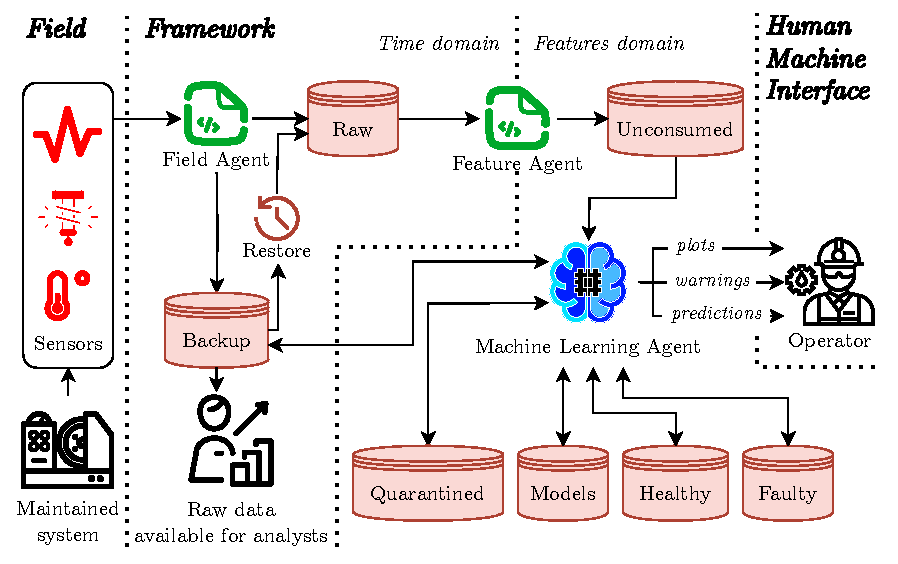
\includegraphics[width=\linewidth]{images/Framework_structure.pdf}
    \caption{The structure of the proposed framework. The Field Agent collects the time series, the Feature Agent extracts the features, and the Machine Learning Agent evaluates the health of the maintained device. The agents are connected to collections of a common database.}
    \label{fig:framework_structure}
\end{figure}

The solution developed in this thesis is thought to be set up on a new device, and linked to the sensors of the most informative quantities of the system.
In the first phase of commissioning, the framework collects the data, extracts the features and stores them. When the data collected is enough to characterize all the modes of operation of the maintained system, the UML model can be trained. Finally, the framework continues collecting new data, extracting the features, and evaluating the new data. The framework now produces a Novelty Metric (NM) that quantifies how abnormal the new data are. 
This phase can last indefinitely. When the NM overshoots a certain threshold, a warning is issued to the maintenance team. 
Then, the team can then decide to perform a maintenance action or to continue monitoring the system. If they declare the system as healthy, the framework can be retrained with the new data, to update the UML model. Otherwise, a second UML model can be trained to characterize the newly discovered fault and perform Fault Detection (FD) in the future.

\subsection{Software Agents}
The proposed framework is based on software agents. Each agent is autonomous and performs a specific task. The developed agents, as shown in Fig.~\ref{fig:framework_structure}, are:
\begin{itemize}
    \item \textbf{Field Agent (FiA)}: responsible for the synchronous sampling of the data. It provides the time series records and ensures a correct sampling frequency.
    \item \textbf{Feature Agent (FA)}: extracts the features from the time series.
    \item \textbf{Machine Learning Agent (MLA)}: trains the UML algorithms and then performs ND, FD and PM. It reports the results to the user.
\end{itemize}

\subsection{Database}
All the Agents are connected to a common database. In the case of the PC implementation, MongoDB has been used. In the case of the Edge implementation, the data are stored directly in the microcontroller's memory.
Regarding the structure shown in Fig.~\ref{fig:framework_structure}, the MongoDB database is composed of seven collections. Every collection has a specific role in the framework. For example, the \emph{Quarantined, Healthy} and \emph{Faulty} collections contain the features that have been flagged as novelty, normal or faulty, respectively.

\subsection{Multiple Instances}
As shown in Fig.~\ref{fig:multiple_instances}, the framework can be implemented in multiple instances. This is useful to better isolate the location of the anomaly in a complex system. The larger the set of sensors that a single instance of the framework is connected to, the more difficult it is to isolate the anomaly. On the other hand, configuring a large group of sensors allows the detection of complex anomalies.

\begin{figure}
    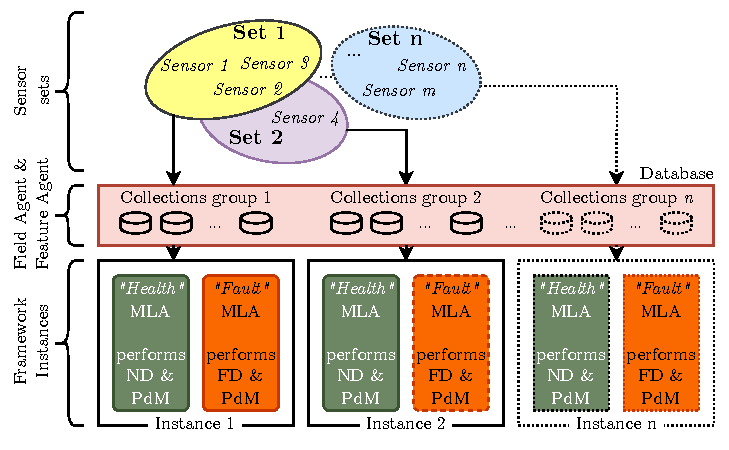
\includegraphics[width=\linewidth]{images/FrameworkInstances.pdf}
    \caption{Multiple instances implementation of the framework. Every instance is linked to a different set of sensors, to monitor different parts of the system.}
    \label{fig:multiple_instances}
\end{figure}


\subsection{Unsupervised Machine Learning Models}

The considered UML implemented in the framework are: \emph{K-means}, \emph{DBSCAN}, \emph{Gaussian Mixture Model} (GMM), \emph{Isolation Forest} (IF), \emph{Local Outlier Factor} (LOF), \emph{One-Class Support Vector Machine} ($\nu$-SVM).

K-means and DBSCAN are traditionally clustering algorithms, so a custom NM has been developed for these algorithms. The other models are already commonly used for ND, so the NM has been linked to the \quoted{score} provided by the library functions.

If the UML is trained with faulty data to perform FD, the NM measures \quoted{how not faulty} the new data are. In this case, the value is transformed into a Fault Metric (FM) with the function $\text{FM} = - \ln(\text{NM} + 1)$ to preserve the coherence. 